\section{图形设备}
SAC支持两种图形设备,分别是xwindows和sgf,默认的图形设备是xwindows。
可以使用 \nameref{cmd:begindevices} 和 \nameref{cmd:enddevices} 命令
开启/关闭指定的图形设备;同时也可以使用 \nameref{cmd:setdevice} 命令
设定默认的图形设备。

\subsection{xwindows}
xwindows即X Window System,也称为X11或X,是一种以位图方式显示的软件
窗口系统。几乎所有的现代操作系统都能支持与使用X,Linux下知名的桌面
环境GNOME和KDE也都是以X窗口系统为基础建构成的。

\begin{figure}[H]
\centering
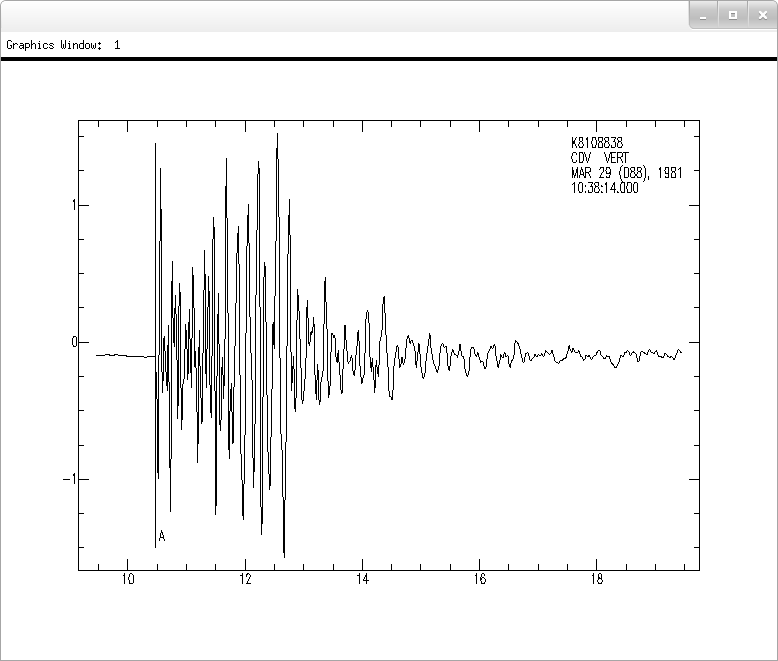
\includegraphics[width=0.9\textwidth]{window}
\caption{SAC绘图窗口}
\label{fig:plot}
\end{figure}

图 \ref{fig:plot} 展示了SAC中的xwindows图形设备的外观,它是SAC默认的
图形设备。同很多其它软件界面类似,xwindows窗口在左上角显示图标,右上角
显示``最小化''、``最大化''、``还原''和``关闭''按钮。窗口的中间部分为
真正的绘图区,本文档的其余插图将只给出绘图区的图像而不再包含窗口部分。

左上角的``Graphics Window: 1''指明了当前绘图窗口的编号为``1'',SAC最多
支持同时打开10个X窗口,编号为1--10。默认情况下只启动并使用1号X窗口。
\nameref{cmd:beginwindow} 命令用于启动指定编号的X窗口;
\nameref{cmd:window} 命令还可以设置每个X窗口的长宽比以及X窗口相对于屏幕
的位置。

\subsection{sgf}
SGF,全称SAC Graphic File,即SAC图形文件,是SAC自定义的一种文件格式,
其包含了绘制一个图件所需要的全部信息,可以通过 \nameref{sec:sgftops}
等工具转换到其它图形设备或图形文件格式。

若启用了SGF图形设备,每次绘制的图件将分别保存到单独的sgf文件中。默认
情况下,sgf图形文件的文件名格式为 !fnnn.sgf! ,其中``nnn''为图件
编号,起始编号为001,每生成一个图件该编号递增。\nameref{cmd:sgf} 命令
可以控制SGF图形设备的选项,比如文件名前缀(默认为 !f!)、
起始编号(默认从 !001! 开始)、保存目录、文件尺寸等。
